\documentclass[rmp,superscriptaddress,10pt,onecolumn]{revtex4-1}
\usepackage[utf8x]{inputenc}
\usepackage{amsmath,amsthm,amsfonts,amssymb,amscd}
\usepackage{graphicx}
\usepackage{wrapfig}
\usepackage{enumerate}
\usepackage{color}
\usepackage[final,
            colorlinks = true,
            linkcolor = blue,
            urlcolor  = blue,
            citecolor = blue]{hyperref}
\usepackage{fontspec}
\usepackage{natbib}
\bibliographystyle{plainnat}
\usepackage{caption}
\usepackage{subcaption}


%\setmainfont{Helvetica}
\usepackage{unicode-math}
\setmathfont{XITS Math}
  \let\oldthefigure\thefigure% Capture figure numbering scheme
  \renewcommand{\thefigure}{S\oldthefigure}% Prefix figure number with S


%\setlength{\parindent}{20pt}
\def\thesubsectiondis{\unskip\arabic{subsection}}
 
\begin{document}

\title{Visualizing and quantifying structural diversity around mobilised AMR genes\\\vspace{3ex} Supplementary Material}
\author{Liam P. Shaw}
\thanks{Correspondence: liam.shaw@biology.ox.ac.uk}
\affiliation{Department of Biology, University of Oxford, Oxford, UK\looseness=-5}
\affiliation{Department of Biosciences, University of Durham, Durham, UK\looseness=-5}
\author{Richard A. Neher}
\affiliation{Biozentrum, University of Basel, Basel, Switzerland\looseness=-5}

\maketitle


\begin{figure}[h]
    \centering
    \includegraphics[width=\linewidth]{figs_supp/FINAL-figs1.pdf}
    % output/pangraph/CTX-M-65/plots/CARD_plot_breakpoint_distances-compare-to-focal-gene.pdf 
    \caption{\textbf{The breakdown of homology in the flanking regions of \textit{bla}$_\mathrm{CTX-M-65}$ and related genes.} As in the main manuscript Fig. 2b, but here we pick only a single isolate for each year/country/genus combination to control for potential sampling bias.}
    \label{fig:CTX-M-65}
\end{figure}

\begin{figure}
     \centering
     \begin{subfigure}[b]{0.45\linewidth}
         \centering
         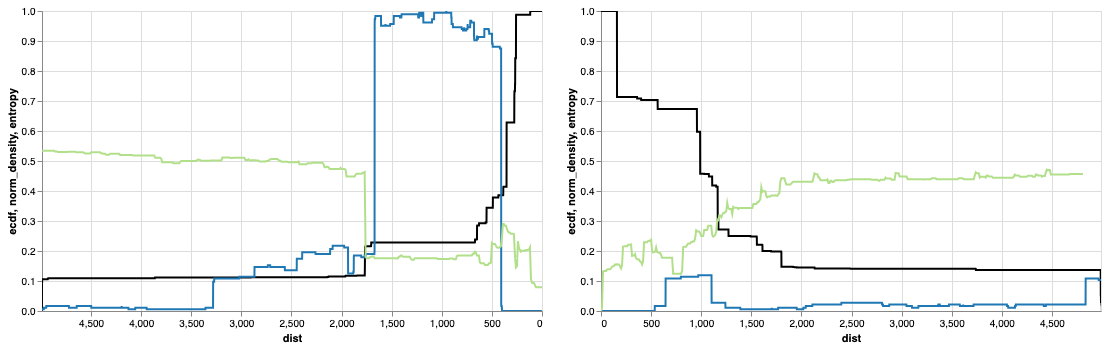
\includegraphics[width=\textwidth]{figs_supp/CMY-2.png}
         \caption{blaCMY-2}
     \end{subfigure}
     \hfill
     \begin{subfigure}[b]{0.45\linewidth}
         \centering
         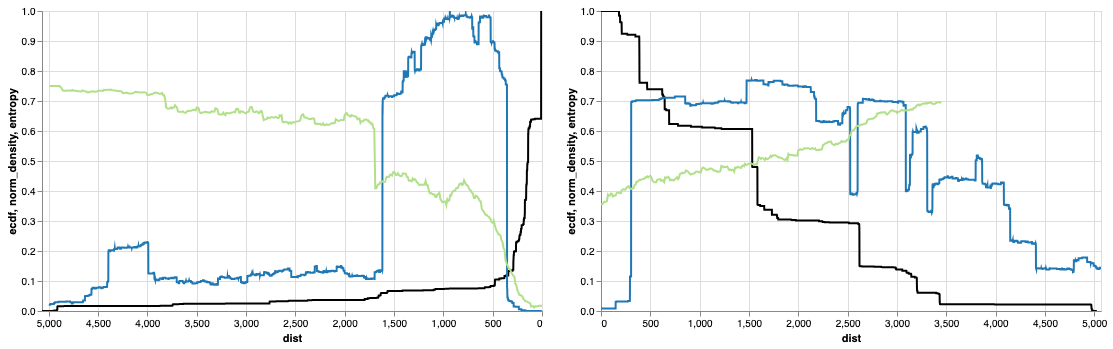
\includegraphics[width=\textwidth]{figs_supp/CTX-M-15.png}
         \caption{blaCTX-M-15}
     \end{subfigure}
     \hfill
     \begin{subfigure}[b]{0.45\textwidth}
         \centering
         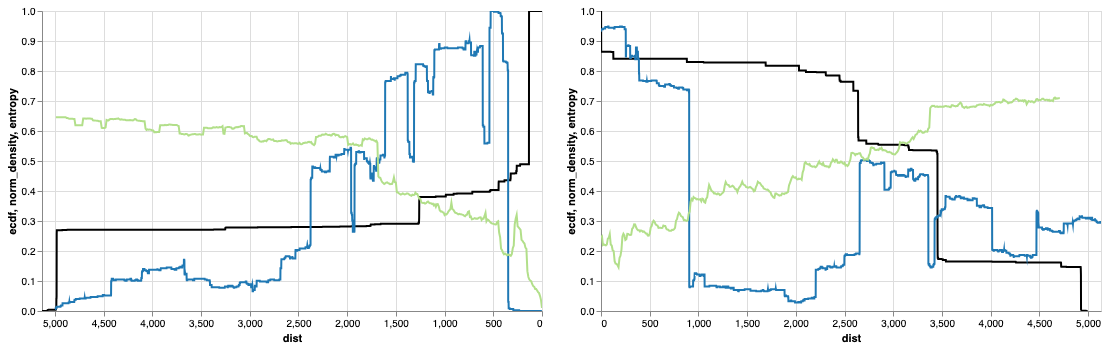
\includegraphics[width=\textwidth]{figs_supp/CTX-M-65.png}
         \caption{blaCTX-M-65}
     \end{subfigure}
          \hfill
     \begin{subfigure}[b]{0.45\textwidth}
         \centering
         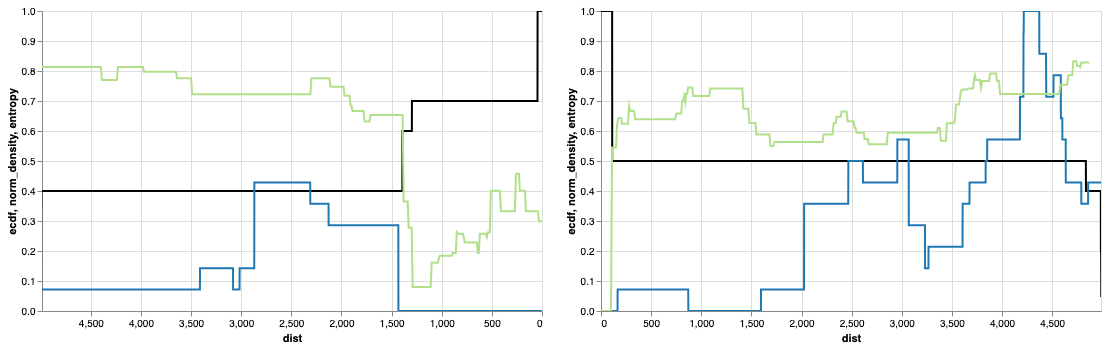
\includegraphics[width=\textwidth]{figs_supp/GES-1.png}
         \caption{blaGES-1}
     \end{subfigure}
          \hfill
     \begin{subfigure}[b]{0.45\textwidth}
         \centering
         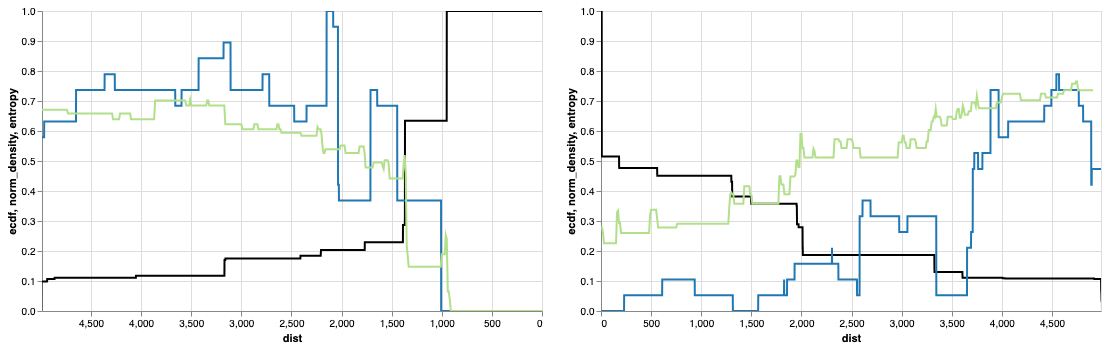
\includegraphics[width=\textwidth]{figs_supp/IMP-4.png}
         \caption{blaIMP-4}
     \end{subfigure}
          \hfill
     \begin{subfigure}[b]{0.45\textwidth}
         \centering
         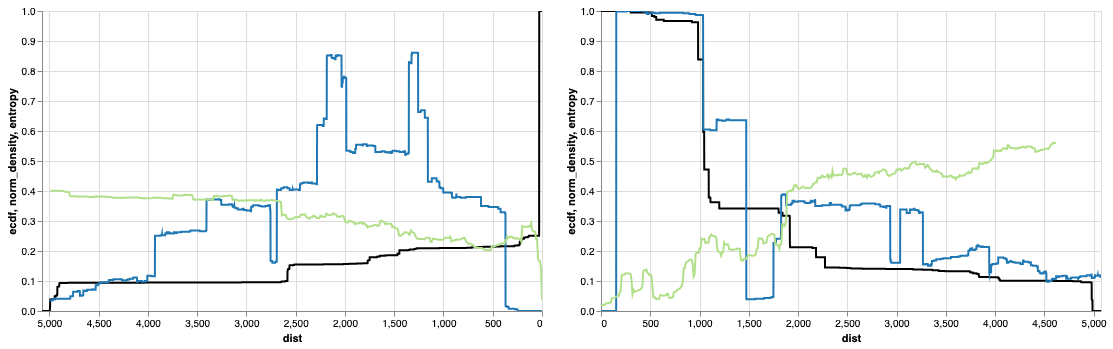
\includegraphics[width=\textwidth]{figs_supp/KPC-2.png}
         \caption{blaKPC-2}
     \end{subfigure}
               \hfill
     \begin{subfigure}[b]{0.45\textwidth}
         \centering
         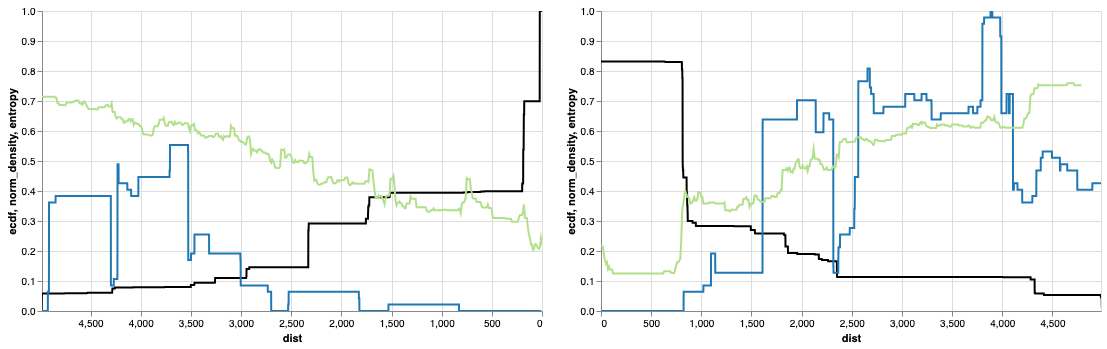
\includegraphics[width=\textwidth]{figs_supp/OXA-10.png}
         \caption{blaOXA-10}
     \end{subfigure}
               \hfill
     \begin{subfigure}[b]{0.45\textwidth}
         \centering
         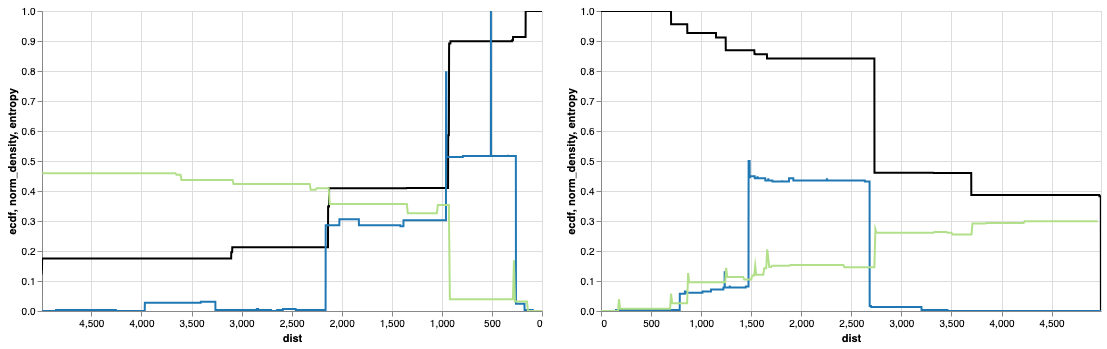
\includegraphics[width=\textwidth]{figs_supp/OXA-48.png}
         \caption{blaOXA-48}
     \end{subfigure}
                    \hfill
     \begin{subfigure}[b]{0.45\textwidth}
         \centering
         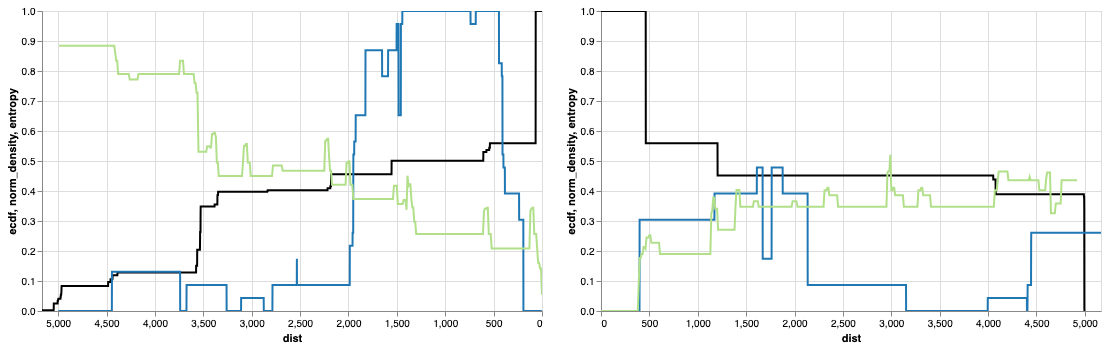
\includegraphics[width=\textwidth]{figs_supp/PER-1}
         \caption{blaPER-1}
     \end{subfigure}
                    \hfill
     \begin{subfigure}[b]{0.45\textwidth}
         \centering
         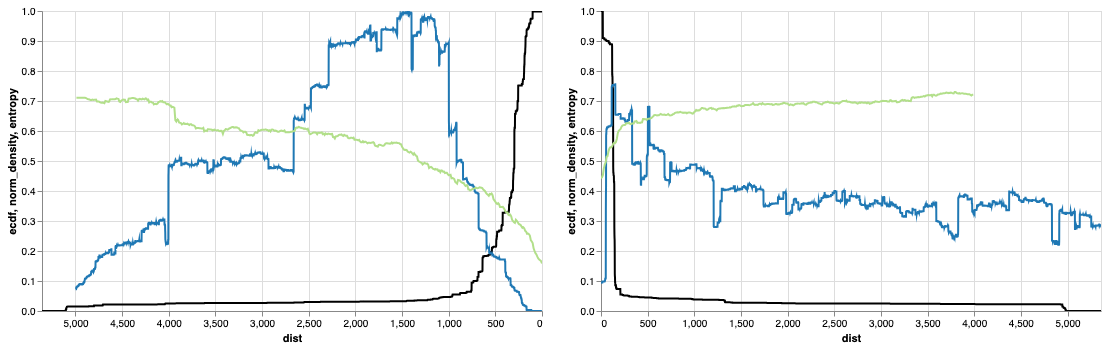
\includegraphics[width=\textwidth]{figs_supp/TEM-1.png}
         \caption{blaTEM-1}
     \end{subfigure}
                    \hfill
     \begin{subfigure}[b]{0.45\textwidth}
         \centering
         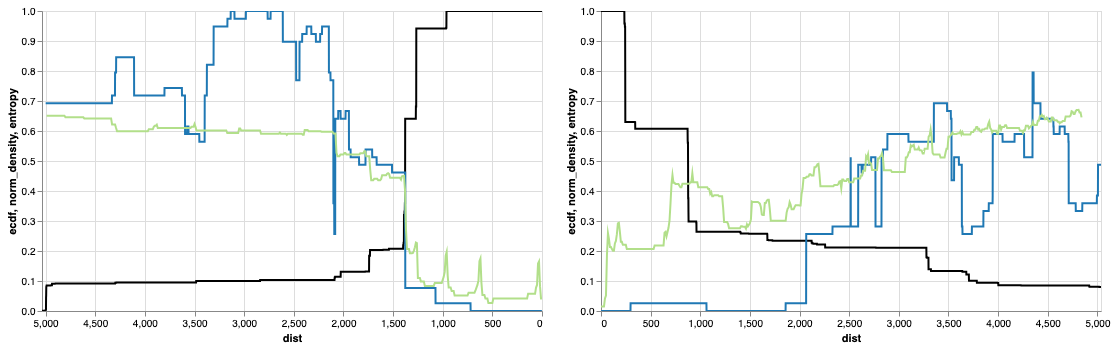
\includegraphics[width=\textwidth]{figs_supp/VIM-1.png}
         \caption{blaVIM-1}
     \end{subfigure}
        \caption{\textbf{Flanking regions of eleven beta-lactamase genes.} Similar to the plot for blaNDM-1 in the main text: overlaid plots of normalised breakpoint distances (black), block diversity (green) and transposase density (blue).}
\end{figure}

\end{document}